\documentclass{article}
\usepackage[utf8]{inputenc}
\usepackage{geometry}
\geometry{top=65px, bottom=65px, left=55px, right=55px}
\usepackage{amsmath}
\usepackage{amssymb}
\usepackage{algorithm}
\usepackage{algorithmic}
\usepackage{indentfirst}
\usepackage{setspace}
\onehalfspacing
\usepackage{url}
\usepackage{hyperref}
\newcommand\tab[1][1cm]{\hspace*{#1}}
\usepackage{listings}
\usepackage{xcolor}
\usepackage{changepage}
\usepackage{graphicx}
\usepackage[pages=some]{background}

\renewcommand{\baselinestretch}{1.15}

\hypersetup{
    colorlinks=true,
    linkcolor=black,
    filecolor=magenta,
    urlcolor=blue,
}

\lstset
{
    breaklines=true,
    breakatwhitespace=true,
    frame=single,
    columns=fullflexible,
    basicstyle=\ttfamily,
    showstringspaces=false,
    %numbers=left,
    %stepnumber=1,
    %numbersep=8pt,
}

\backgroundsetup{
scale=1,
color=black,
opacity=0.05,
angle=10,
position={12cm,-22cm},
contents={%
  
\includegraphics[height=20cm,width=20cm,keepaspectratio]{images/sceau.jpg}
  }%
}

%\newcommand\tab[1][1cm]{\hspace*{#1}}
\newcommand\bld[1]{\textbf{#1}}
\newcommand\ita[1]{\textit{#1}}
\newcommand\pcw[1]{\texttt{#1}}

\begin{document}
\begin{titlepage}
    \begin{center}
        \BgThispage
        \vspace*{1cm}
        
        
        \huge
        \textbf{Data Warehouses}
        \vspace{0.25cm}
        
        \LARGE
        \textbf{INFO-H419}
        
        \vspace{0.5cm}
        \LARGE
        {Part 1 : TPC-DS benchmark on Impala}
        
        
        \vspace{3.5cm}
        
        \textbf{BAKKALI Yahya (000445166) \\}
        \textbf{FALLAHI Amirmohammad (000460073) \\}
        \textbf{HAUWAERT Maxime (000461714) \\}
        \textbf{LIBERT Alexandre (000435755) \\}
    
        \vspace{2.5cm}
        \textit{October 2021 \\}
        \vspace{0.5cm}
        \textsc{Université Libre de Bruxelles (ULB)}
        
        
    \end{center}
\end{titlepage}

\tableofcontents
\thispagestyle{empty}
\newpage
\setcounter{page}{1}
\setlength{\parskip}{1em}

\section{Introduction}
Databases are inseparable parts of programming and today's technologies. As the quantity of data are increasing constantly, using an efficient database is the main key to overcome the problem of analyzing the data and getting answers in reasonable amounts of time.

Since there exist a lot of different databases, choosing one which is efficient in answering the queries related to a specific domain is a hard task. Therefore, database \bld{benchmarks} can be used in order to compare efficiency and performance of different databases. A database benchmark is a repeatable experimentation on performance of database in various fields such as memory occupation or execution time. 

\bld{TPC} is one of the corporation which focused on developing databases benchmark standards. One of the benchmarks that TPC provided is \bld{TPC-DS} benchmark. TPC-DS is a decision support benchmark that simulates numerous components of a decision support system, such as queries and data maintenance.

In this paper the details of the TPC-DS experiment performed on \bld{Impala} will be seen. Apache Impala is the open source, native analytic database for Apache Hadoop.

\section{Hardware specification}
In order to do the benchmark experimentation, the \ita{Dell xps-15-9560} computer has been used. The following table show the hardware specification of this computer.

\begin{table}[h]
\centering
\begin{tabular}{|l|c|}
\hline
Operating system & Ubuntu 20.04.3 LTS \\ \hline
System type & 64 bits \\ \hline
CPU & Intel®Core™i7-7700HQ \\ \hline
CPU frequency & 2.8 GHz up to 3.8 GHz \\ \hline
RAM capacity & 16 GB \\ \hline
RAM type & DDR4 \\ \hline
RAM speed & 2,400 MT/s \\ \hline
Hard disk & PM981 NVMe Samsung \\ \hline
Hard disk capacity & 256 GB \\ \hline
\end{tabular}
\caption{Device information}
\label{table:Table 1}
\end{table}


\section{Software specification}
In this section, details about Impala, its installation and its functioning will be seen. In order to facilitate reproduction of the experimentation, some scripts have been written, which will be explained in the upcoming sections. It is also necessary to mention that for this experimentation Impala \bld{version 4.0.0} has been used.  

\subsection{Apache Impala}
Apache Impala is an open-source SQL query engine which uses massively parallel computing \footnote{Massively Parallel computing is a way of computing in which numerous computers (CPUs) work simultaneously in parallel to execute a group of computations} for data stored in an Apache Hadoop distribution. It provides SQL queries with great speed and minimal latency. When working with medium-sized datasets is required, and real-time responses are necessary, Impala is the ideal solution.

\subsection{Impala's prerequisites}
In order to work with impala, knowing the basics of Apache Hadoop, HDFS (Hadoop Distributed File System) commands and basic knowledge of SQL is required. HDFS is the Hadoop significant component, in charge of storing enormous datasets of structured or unstructured data across several nodes and as result of that, maintaining metadata in log files format. The following table shows some HDFS commands, their description, and their \ita{UNIX} equivalence (if it exists.)


\begin{table}[h]
\centering
\begin{tabular}{|c|c|c|}
\hline
HDFS command & Description & UNIX equivalent \\ \hline \hline
ls & List all files & ls \\ \hline
lsr & Same as ls but with recursive perspective & ls -R \\ \hline
mkdir & Create a directory & mkdir \\ \hline
touchz & Create an empty file & touch \\ \hline
cat & Print file contents & cat \\ \hline
copyFromLocal (put) &  Copy files or directories from OS to hdfs store & $\varnothing$ \\ \hline
copyToLocal (get) & Copy files or directories from hdfs store to OS &  $\varnothing$ \\ \hline
moveFromLocal & Move file from OS to hdfs & $\varnothing$ \\ \hline
cp  & Copy files & cp \\ \hline
mv & Move files & mv \\ \hline
rmr & Delete a file from HDFS recursively & rm -r \\ \hline
du & Give the size of each file in directory & ls -s \\ \hline
\end{tabular}
\caption{HDFS basic commands}
\label{table:Table 2}
\end{table}



\subsection{Installing Impala}
Impala can be installed by using the source code of their official GitHub repository\footnote{\url{https://github.com/apache/impala}}.
Once the repository had been cloned, the following instructions can be used to install Impala on the system\footnote{\url{https://cwiki.apache.org/confluence/plugins/servlet/mobile?contentId=65146982\#content/view/65146982}}.
\vspace{0.5cm}
\begin{lstlisting}[language=bash]
$ git clone https://gitbox.apache.org/repos/asf/impala.git ~/Impala
$ cd ~/Impala
$ export IMPALA_HOME=`pwd`
$ ./bin/bootstrap_system.sh
$ source ./bin/impala-config.sh
$ ./buildall.sh -noclean -notests -format -start_minicluster -start_impala_cluster
\end{lstlisting}

The last step took at least one hour to complete.
% Then each time the computer is restarted, a custom script, which is based on the build script of the repository, is used to start impala. The advantage of using this script, is that it will not delete all the data that have been inserted.

This script first initializes all the environments variables, then it starts following services:

\begin{itemize}
\item Apache Hadoop : consisting of a storage part; HDFS (Hadoop Distributed File System), a processing part and the MapReduce. Hadoop divides files into large blocks and distributes them on cluster nodes.
\item Apache YARN (Yet Another Resource Negotiator) : which is the Hadoop cluster manager.
\item Apache Kudu : is the Hadoop ecosystem columnar data-store optimized to use on memory-intensive hardware.
\end{itemize}

Finally, it starts an Impala Cluster running with 3 nodes (3 coordinators, 3 executors).


\subsection{Launching Impala}
Once the impala build has been successfully performed, the impala cluster will be started and connected automatically. However, after each reboot of the computer, the following commands must be executed to start the cluster and establish the connection with impala. Before launching it, some important variables must be set. The script \textbf{impala-config.sh} can be used for this aim.

\vspace{0.5cm}
\begin{lstlisting}[language=bash]
$ cd ~/Impala
$ source bin/impala-config.sh
$ testdata/bin/run-all.sh
$ bin/start-impala-cluster.py
\end{lstlisting}

\subsection{Interacting with Impala}
There exists a lot of ways to interact with Impala. The easiest method, which was used in this project, is to simply use the \textbf{Impala-Shell} program. The shell can be launched by using this command.

\vspace{0.5cm}
\begin{lstlisting}[language=bash]
$ bin/impala-shell.sh
\end{lstlisting}

The \textbf{Impala-Shell} program can also execute a query directly given in the command.
\vspace{0.5cm}
\begin{lstlisting}[language=bash]
$ bin/impala-shell.sh -f <SQL file> -d <database name>
\end{lstlisting}

\subsection{TPC}
TPC is a corporation which establishes and develops objective transaction processing and databases benchmarks. In this part of the project, TPC-DS is used to verify performance and efficiency of Impala. TPC-DS benchmark illustrates decision support systems that :
\begin{itemize}
    \item Analyze enormous amounts of data
    \item Provide solutions to real-world business problems
    \item Execute queries with a variety of operational needs and complexity
    \item Are marked by a high CPU and IO load.
    \item Are regularly with source OLTP databases by using maintenance functions.
    \item Launch on \bld{Big Data} solutions, like RDBMS and also Hadoop/Spark based systems.
\end{itemize}

\section{Implementation}
In this section, details of implementation and experimentation will be seen. This section shows how the input of the experimentation has been provided and also explains how the situation of the experimentation has been facilitated for users. 

\subsection{TPC-DS kit}
In order to launch the experimentation, TCP-DS tool was downloaded from TCP official website\footnote{\url{http://tpc.org/tpc_documents_current_versions/current_specifications5.asp}}.
\subsubsection{Data generation}
The TPC-DS kit provides a data population generator to generate experimental data for different scaling factors. The command line executed for this purpose is as follows:
\vspace{0.5cm}
\begin{lstlisting}[language=bash]
$ ./dsdgen -scale <volume of datae> -dir <output destination> -parallel 4 -child 1 &
$ ./dsdgen -scale <volume of data> -dir <output destination> -parallel 4 -child 2 &
$ ./dsdgen -scale <volume of data> -dir <output destination> -parallel 4 -child 3 &
$ ./dsdgen -scale <volume of data> -dir <output destination> -parallel 4 -child 4
\end{lstlisting}

\subsubsection{Queries generation}

To perform the benchmark and obtain the results of the experimentation, the TPC-DS model queries have been adapted to obtain executable \pcw{.sql} queries on Impala. The TPC-DS tool has dialects to convert the model queries into SQL queries, the ``netezza" dialect is the closest to Impala, however the dialects given with the tools do not work until the following line is added at the end of these files ``define \_END = ``";". The following bash codes show how to generate the 99 queries.

%Then the following bash codes have been executed in order to obtain \pcw{.sql} queries from the TPC-DS tool. 

\vspace{0.5cm}
\begin{lstlisting}[language=bash]
$ for i in {1..99};
> do 
> ./dsqgen -template query$i.tpl -directory <query_templates directory of TPC-DS tool> -output <output destination> -dialect netezza -scale <volume of data>; 
> mv <output destination/query_0.sql> <output destination/query_$i.sql>;
> done
\end{lstlisting}


%These queries have been used as the inputs of experimentation to achieve the benchmark result.

\subsection{Scripts}

The following scripts have been implemented in order to make the experimentation simplier.

\subsubsection{create\_tables.sql}

This script was provided by TPC corporation in order to initialize the experimentation by creating table. As the experimentation have been performed on Impala, this script has been changed a little bit in order to be compatible with Impala; It is a simple script which creates tables with the aim of collecting the experimentation data.

\subsubsection{execute\_queries.sh}



As there are 99 queries, it would be time-consuming to execute the queries one by one; So, a script has been implemented in order to automate the execution of TPC queries and starts the examination. For each execution, its output will be stored in a distinct file and its execution time will be appended to a file which records execution time.
\vspace{0.5cm}
\begin{lstlisting}[language=bash]
$ ./execute_queries.sh <query_path_older> <answer_path_folder>
\end{lstlisting}

\subsubsection{load\_data.sh}

This script loads data in the tables that we created by \pcw{create\_tables.sh}; It uses \pcw{moveFromLocal} command of \ita{HDFS} in order to move files from local path (OS) to HDFS (Hadoop Distributed File System). The following box shows the code that have been executed for each table :
\vspace{0.5cm}
\begin{lstlisting}[language=bash]
$ hdfs dfs -moveFromLocal <data_source>/<table_name>.dat <data_destination>/<table_name>;
\end{lstlisting}


\subsection{Queries adaptation}
As Impala is different a little bit from original \ita{SQL}, some of the queries have been updated in order to be compatible with impala. These adaptions are as follows:
\subsubsection{Type A: Date and INTERVAL keyword} 
In this type of adaptation, the date syntax errors have been handled. The time syntax in the template queries is not valid for Impala. It was therefore necessary to use vendor specific syntax for date expressions and date casting in some cases. 

\begin{tabular}{p{8cm}|p{8cm}}

\hspace{3cm} Before & \hspace{3cm} After \\

\begin{lstlisting}[frame=none, escapechar=!]
where date_sk = d_date_sk and d_date between cast('[SALES_DATE]' as date) and (cast('[SALES_DATE]' as date) +  !\colorbox{red}{14 days}!) and store_sk = s_store_sk
\end{lstlisting}

&

\begin{lstlisting}[frame=none, escapechar=!]
where date_sk = d_date_sk and d_date between cast('[SALES_DATE]' as date) and (cast('[SALES_DATE]' as date) +  !\colorbox{green}{INTERVAL 14 days}!) and store_sk = s_store_sk
\end{lstlisting} 

\end{tabular}

\subsubsection{Type B: ORDER BY instruction followed by CASE WHEN keyword}

The aliases after keyword ``CASE WHEN" which has been implemented in an ``ORDER BY" instruction, are unknown to Impala; Therefore, in this adaptation type, these kind of aliases have been replaced by their initial values.

\begin{tabular}{p{8cm}|p{8cm}}

\hspace{3cm} Before & \hspace{3cm} After \\

\begin{lstlisting}[frame=none, escapechar=!]
 [_LIMITA] select [_LIMITB]
    ...
   ,grouping(i_category)+grouping(i_class) as lochierarchy
   ...
 from
   ...
 where
   ...
 group by rollup(i_category,i_class)
order by
   lochierarchy desc
  ,case when !\colorbox{red}{lochierarchy}! = 0 then i_category end
  ,rank_within_parent
  [_LIMITC];
\end{lstlisting}

&

\begin{lstlisting}[frame=none, escapechar=!]
 [_LIMITA] select [_LIMITB]
    ...
   ,grouping(i_category)+grouping(i_class) as lochierarchy
   ...
 from
   ...
 where
   ...
 group by rollup(i_category,i_class)
order by
   lochierarchy desc
  ,case when !\colorbox{green}{grouping(i\_category)+grouping(i\_class)}! = 0 then i_category end
  ,rank_within_parent
  [_LIMITC];
\end{lstlisting}

\end{tabular}


\subsubsection{Type C: Nested table expressions} 

As Impala does not allow to use nested table expressions without giving name to interior expressions, this adaption type have been considered in order to settle this problem.

\begin{tabular}{p{8cm}|p{8cm}}

\hspace{3cm} Before & \hspace{3cm} After \\

\begin{lstlisting}[frame=none, escapechar=!]
 with wscs as
 (  select sold_date_sk, sales_price
    from (  select ws_sold_date_sk sold_date_sk, ws_ext_sales_price sales_price
            from web_sales 
            union all
            select cs_sold_date_sk sold_date_sk, cs_ext_sales_price sales_price
            from catalog_sales !\colorbox{red}{))}!,
\end{lstlisting}

&

\begin{lstlisting}[frame=none, escapechar=!]
 with wscs as
 (  select sold_date_sk, sales_price
    from (  select ws_sold_date_sk sold_date_sk, ws_ext_sales_price sales_price
            from web_sales 
            union all
            select cs_sold_date_sk sold_date_sk, cs_ext_sales_price sales_price
            from catalog_sales !\colorbox{green}{) AS tmp)}!,
\end{lstlisting}

\end{tabular}

\subsubsection{Type D: Reserved keywords} 

As the templates queries sometimes used some reserved keywords of \ita{SQL}, this adaption type have been defined; The character ``\textasciigrave" have been used around these words in order to transform them to normal aliases

\begin{tabular}{p{8cm}|p{8cm}}

\hspace{3cm} Before & \hspace{3cm} After \\

\begin{lstlisting}[frame=none, escapechar=!]
select s_store_id, sum(sales_price) as sales, sum(profit) as profit, sum(return_amt) as !\colorbox{red}{returns}!, sum(net_loss) as profit_loss
\end{lstlisting}


&

\begin{lstlisting}[frame=none, escapechar=!]
select s_store_id, sum(sales_price) as sales, sum(profit) as profit, sum(return_amt) as !\colorbox{green}{\textasciigrave returns\textasciigrave}!, sum(net_loss) as profit_loss
\end{lstlisting} 

\end{tabular}


\subsubsection{Type E: Alternatives} 

The queries number 10 and 35 could not be adapted to perform by Impala, therefore alternative version of these queries provided by \ita{TPC-DS}, have been used.

\subsubsection{All the adaptions in one sight}

The following table shows all the queries that have been modified according to one of the types above;  
\begin{table}[H]
\centering
\begin{tabular}{|c|c|}
\hline
Adaption type & Queries number \\ \hline \hline
Type A &  5, 12, 16, 20, 21, 32, 37, 40, 72, 77, 80, 82, 92, 94, 95, 98 \\ \hline
Type B & 36, 70, 86 \\ \hline
Type C & 2, 14, 23, 49 \\ \hline
Type D & 5, 77, 80, 99 \\ \hline
Type E & 10, 35 \\ \hline
\end{tabular}
\caption{Queries adaption}
\label{table:Table 3}
\end{table}


\section{Benchmark results and analysis}

In this section, the different benchmarks done as well as their results and some analysis will be seen.

It has been decided to set the size of the biggest data-set to 50 GB due to limited storage capacity, which represents the reference scale factor 1.0. Three other scale factors have been chosen, 0.02, 0.2 and 0.5, which give three datasets of size 1, 10, 25 GB in addition to the 50 GB one.

For each of the scale factor, the queries have been re-generated as described in the queries generation section.

In order to have more precise and reliable result, for each data-set the queries have been executed six times and the displayed result is the average of the last five executions. Except for the 50 GB data execution, where the queries have been run only once due to time related issues.

The four following figures \ref{ExecutionTime1GB}, \ref{ExecutionTime10GB}, \ref{ExecutionTime25GB} and \ref{ExecutionTime50GB} show the execution time of each query on the four datasets. It was chosen to show these results using this kind of chart instead of the typical histogram used in this type of situation, as they are more appropriate.

\subsection{Experiment 1 : 1 GB dataset}

\begin{figure}[H] 
\begin{adjustwidth}{-2cm}{-2cm}
\begin{center}
%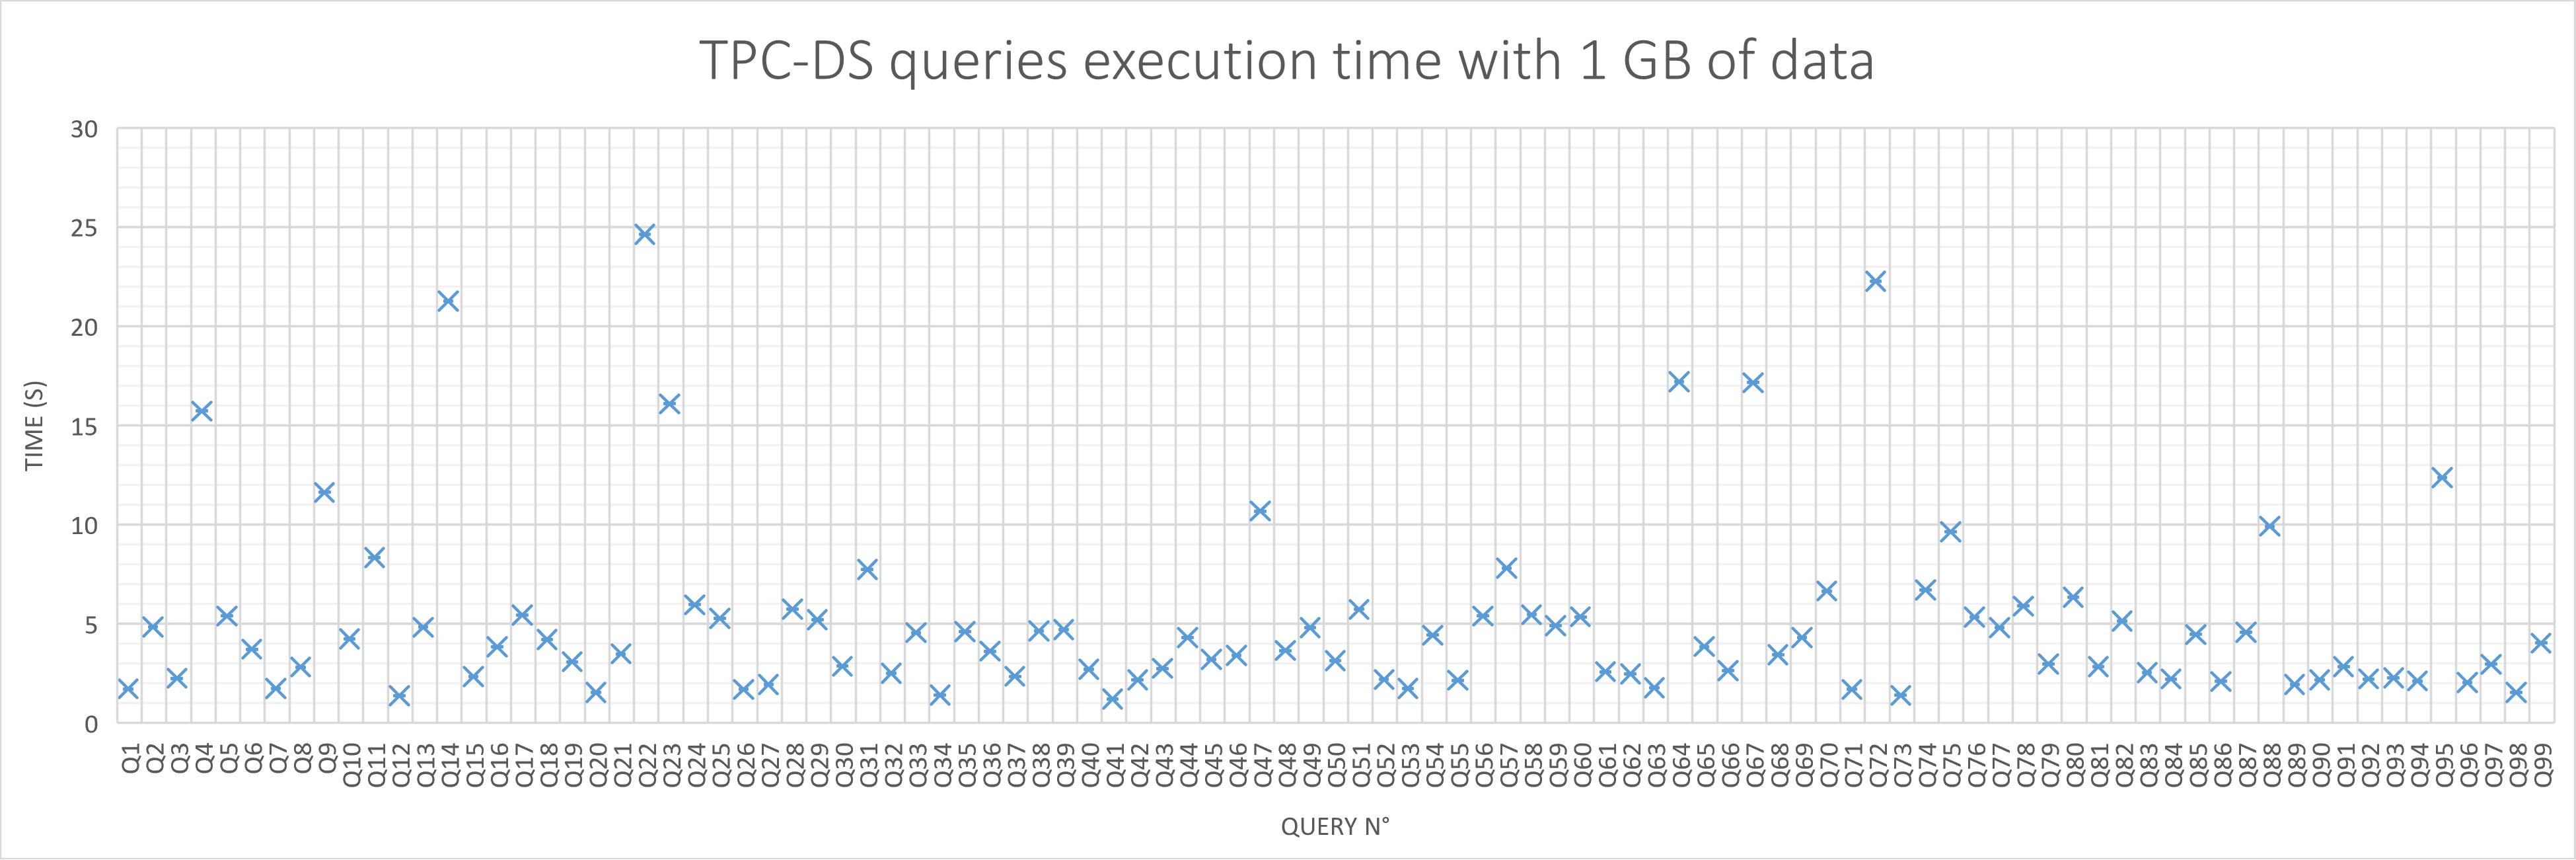
\includegraphics[width=17.5cm, height=6.5cm]{images/ExecutionTime1GB.png}
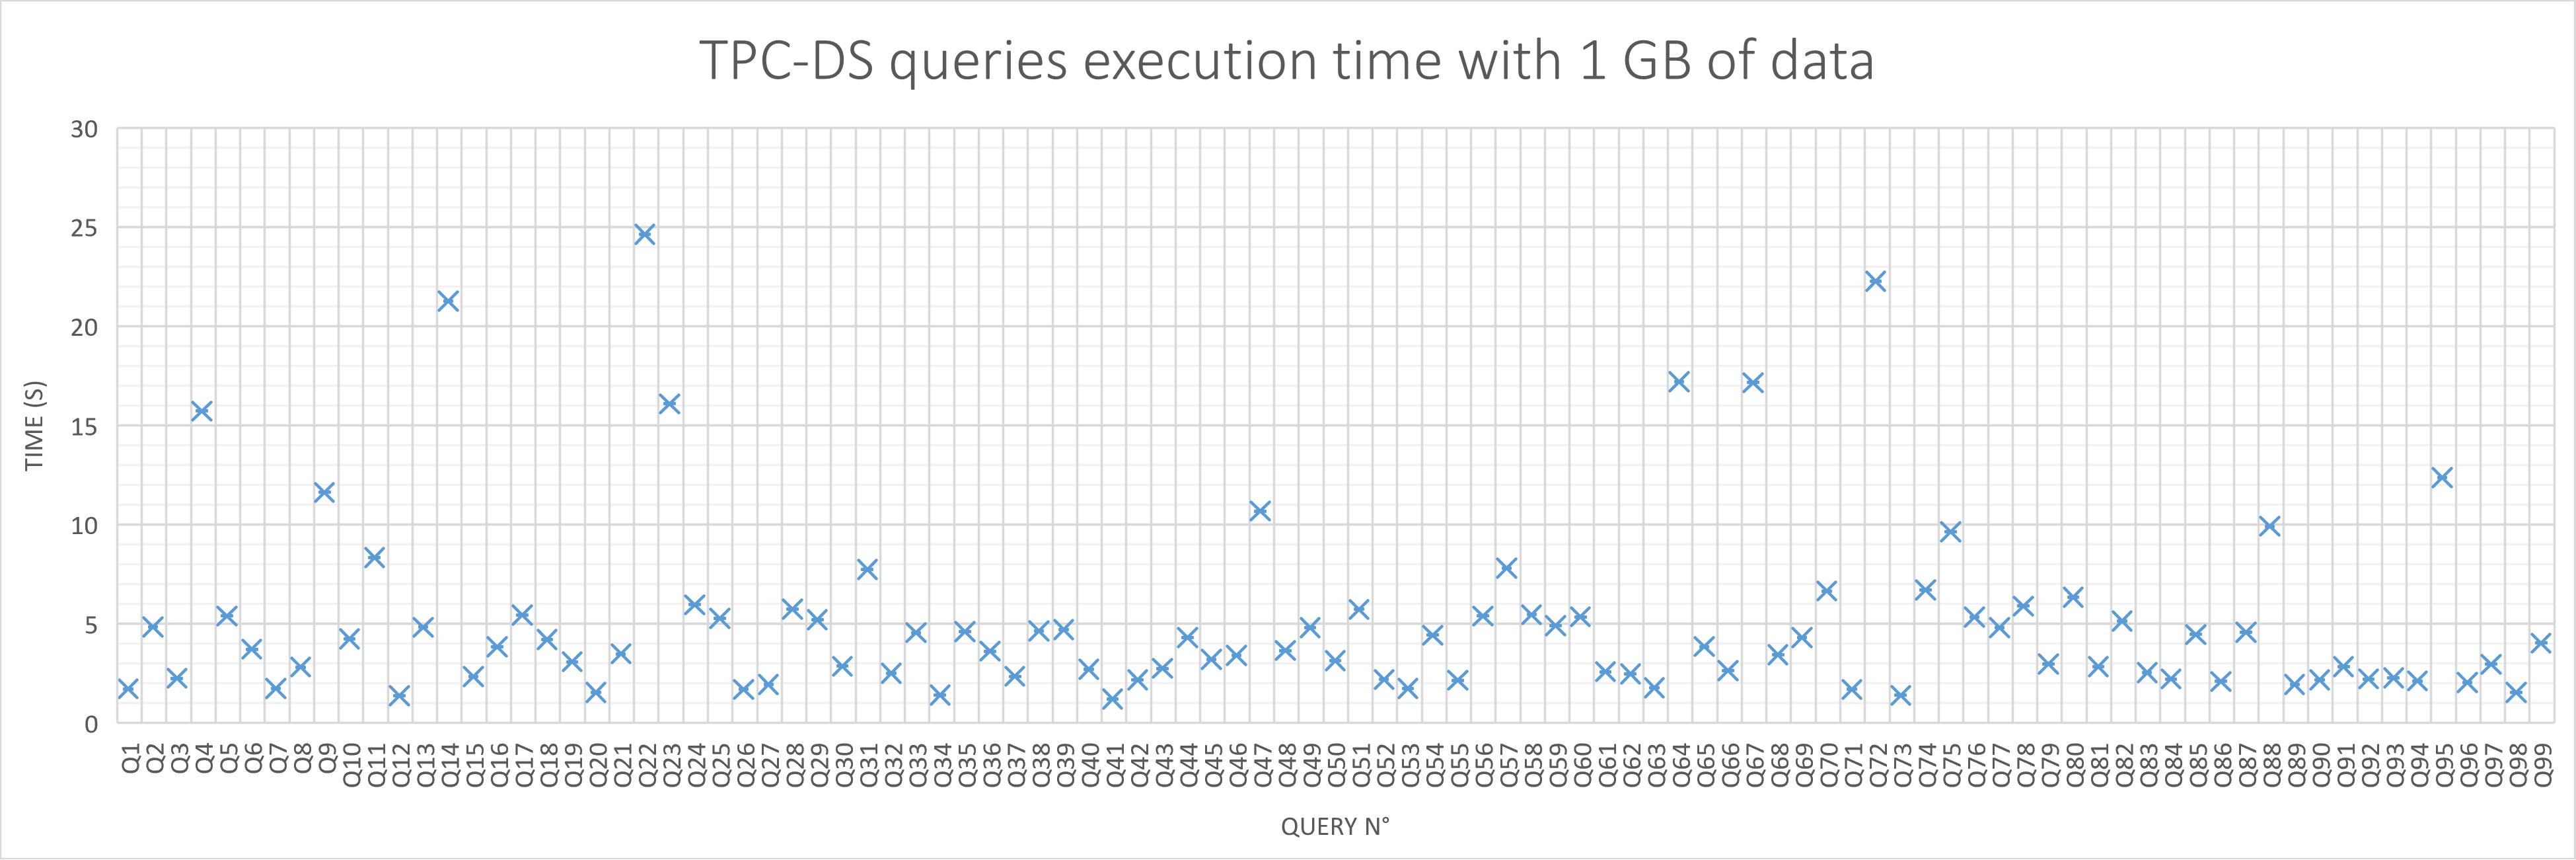
\includegraphics[width=20cm]{images/ExecutionTime1GB.png}
\end{center}
\end{adjustwidth}
\caption{Execution time with 1 GB of data}
\label{ExecutionTime1GB}
\end{figure}

It can be seen that the execution time of the 99 queries vary between 1.22 and 24.64 secs, the average execution time is equal to 5.12 secs. Some queries take a lot of time, up to 4 or 5 times more than the average ones. The overall execution time of all the queries is equal to 506.61 s.



\subsection{Experiment 2 : 10 GB dataset}

\begin{figure}[H]
\begin{adjustwidth}{-2cm}{-2cm}
\begin{center}
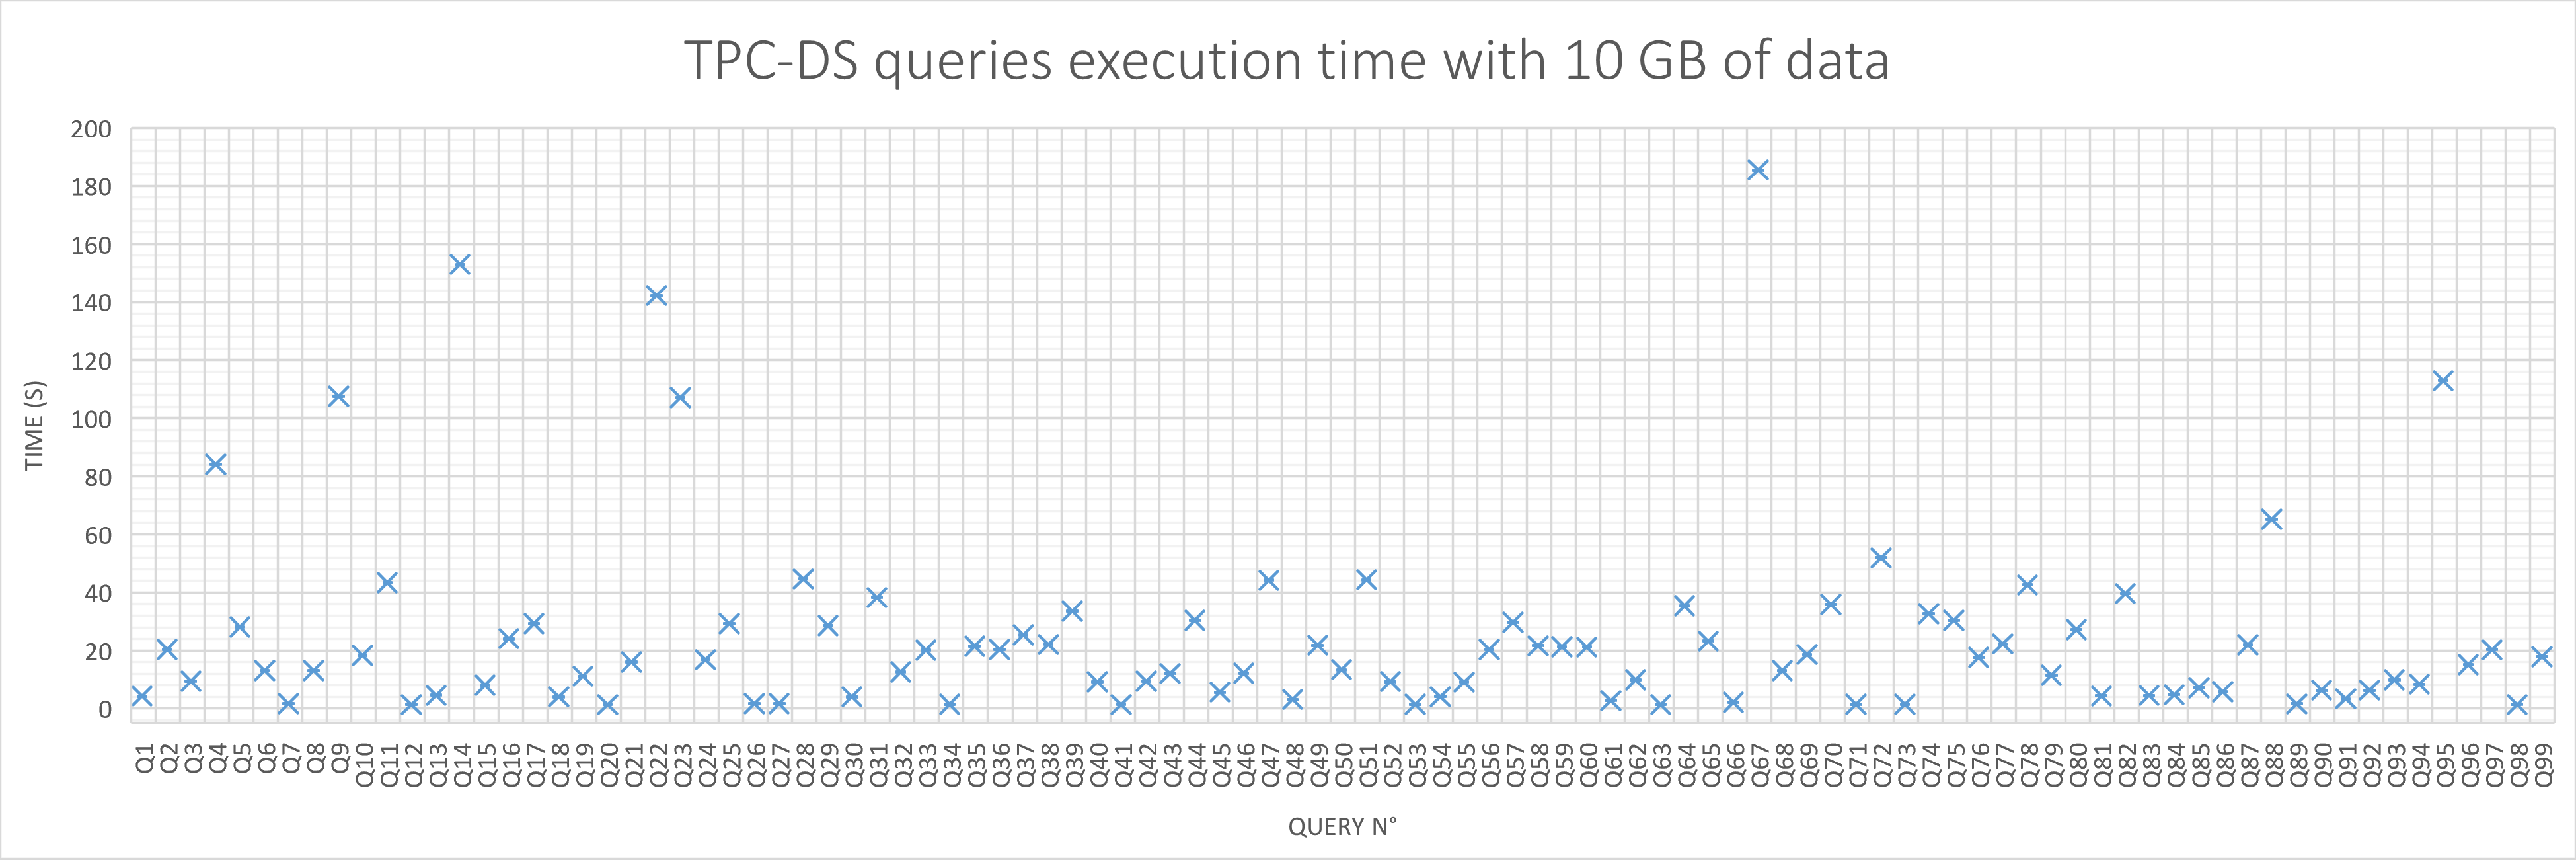
\includegraphics[width=20cm]{images/ExecutionTime10GB.png}
\end{center}
\end{adjustwidth}
\caption{Execution time with 10 GB of data}
\label{ExecutionTime10GB}
\end{figure}

It can be seen that the execution time of the 99 queries vary between 1.38 and 185.54 secs, the average execution time is equal to 24.63 s. Some queries take a lot of time, up to 4 or 5 times more than the average ones. The overall execution time of all the queries is equal to 2438.59 s.

%\subsubsection{All adaptions in one sight}

\subsection{Experiment 3 : 25 GB dataset}

\begin{figure}[H] 
\begin{adjustwidth}{-2cm}{-2cm}
\begin{center}
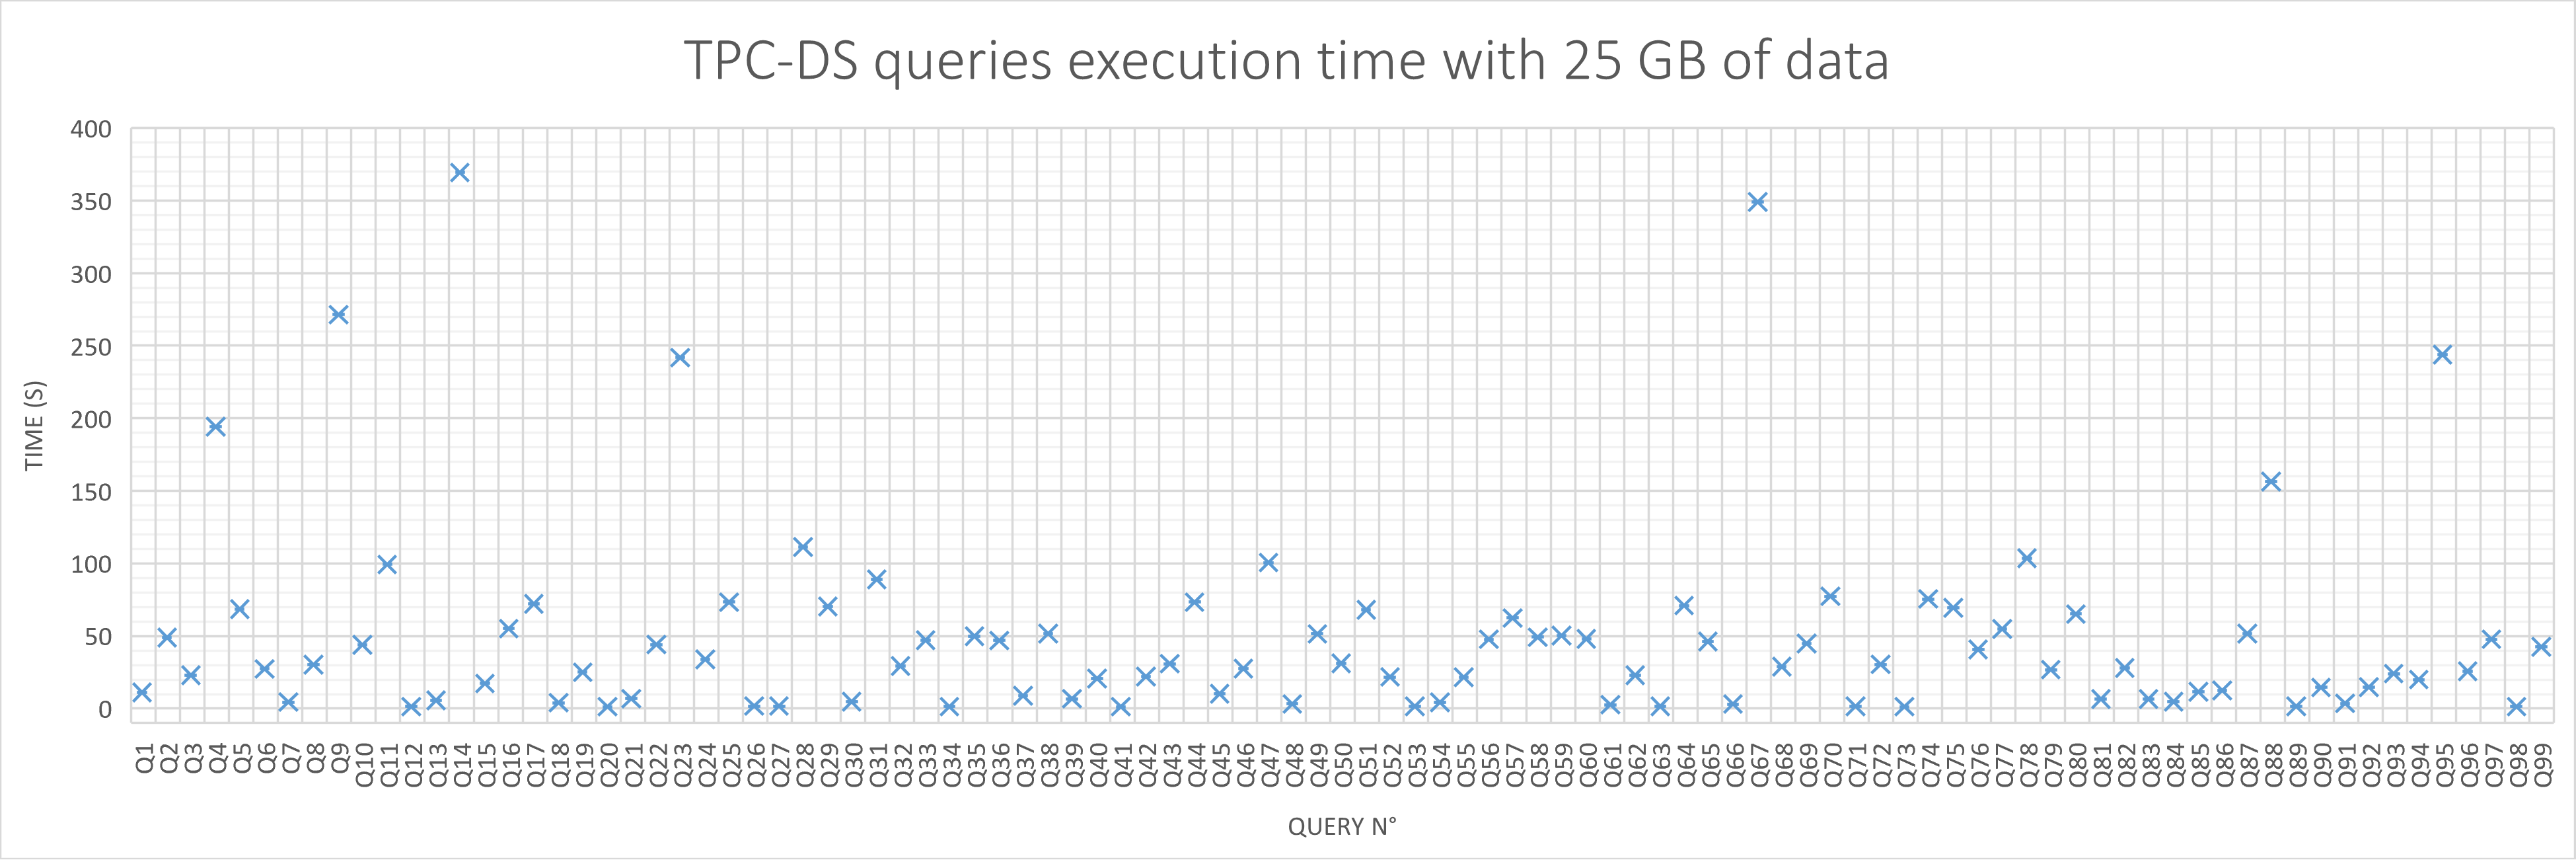
\includegraphics[width=20cm]{images/ExecutionTime25GB.png}
\end{center}
\end{adjustwidth}
\caption{Execution time with 25 GB of data}
\label{ExecutionTime25GB}
\end{figure}

It can be seen that the execution time of the 99 queries vary between 1.29 and 369.31 secs, the average execution time is equal to 49.28 secs. Some queries take a lot of time, up to 4 or 5 times more than the average ones. The overall execution time of all the queries is equal to 4878.49 s.

\subsection{Experiment 4 : 50 GB dataset}

\begin{figure}[H] 
\begin{adjustwidth}{-2cm}{-2cm}
\begin{center}
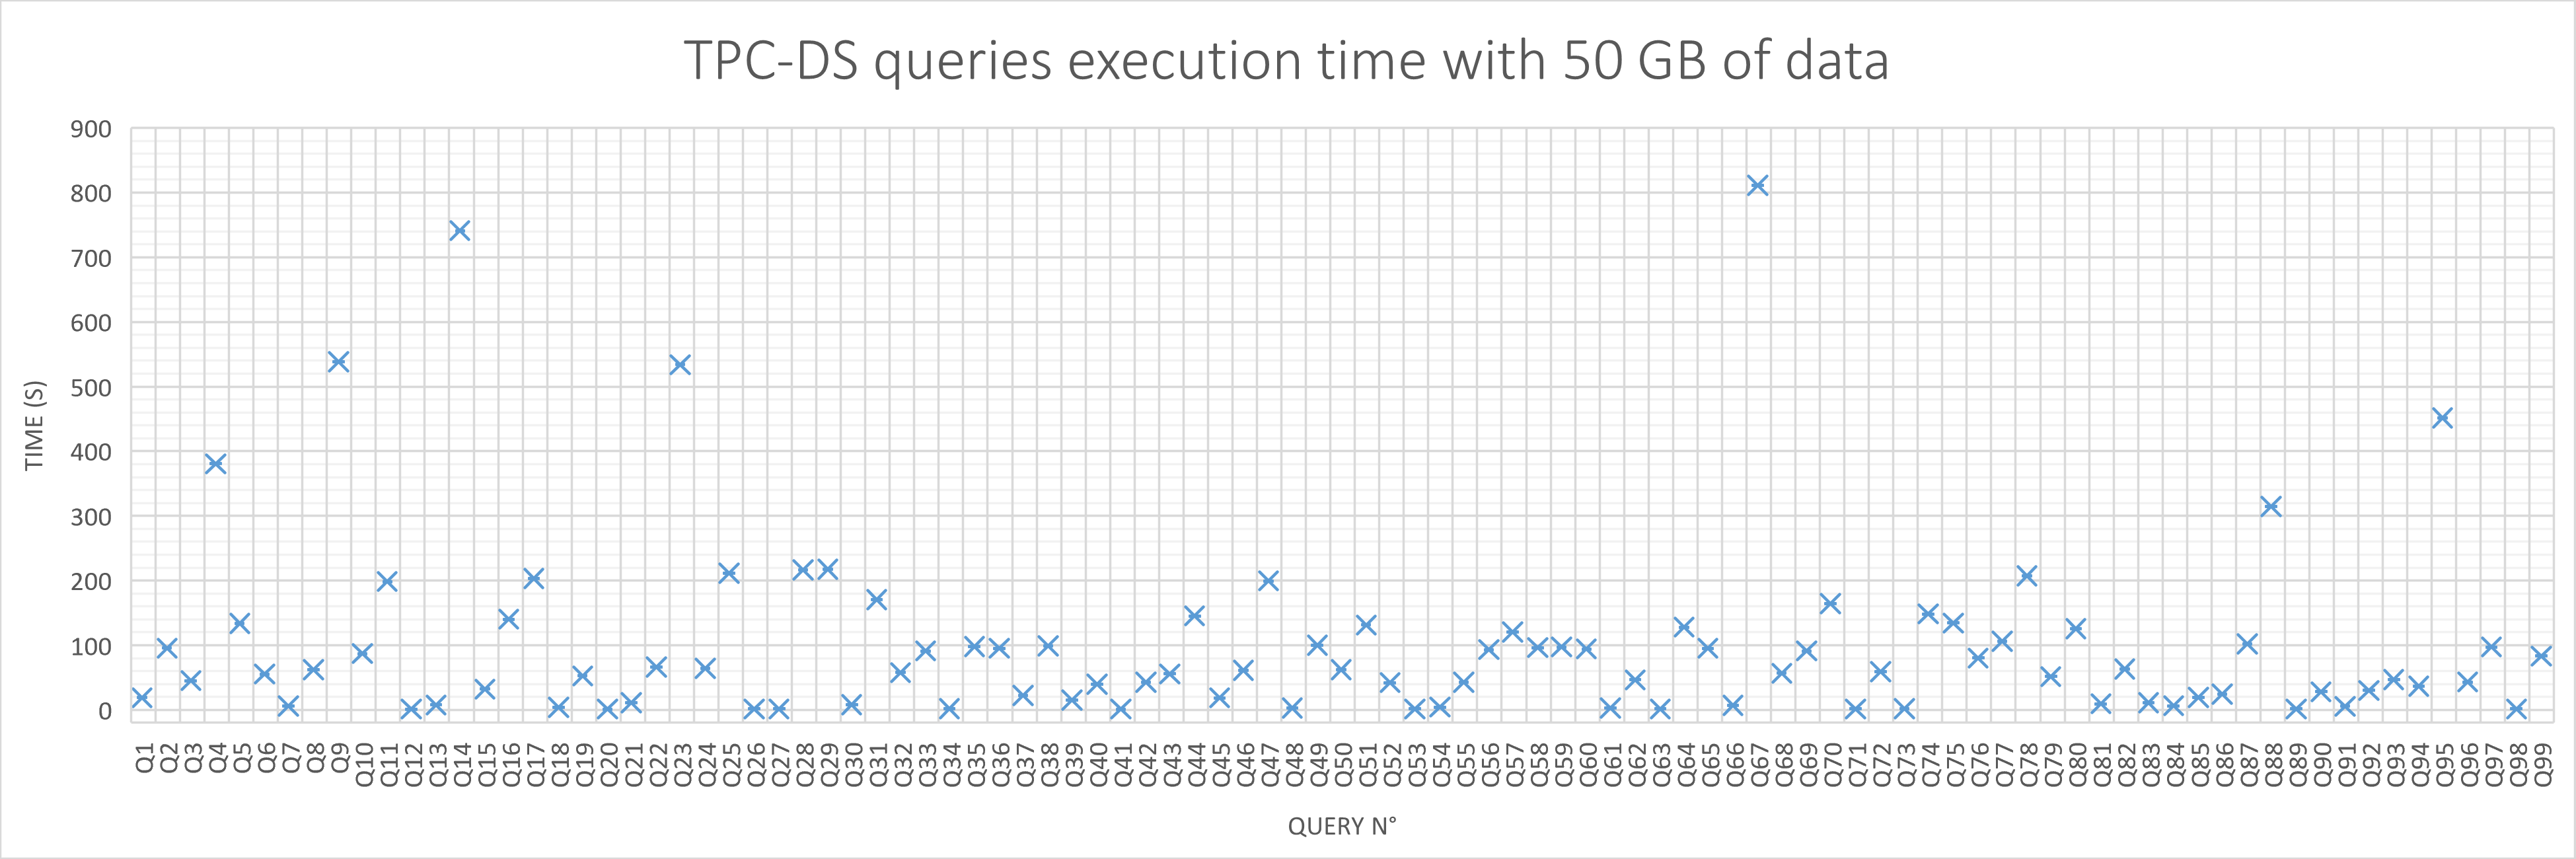
\includegraphics[width=20cm]{images/ExecutionTime50GB.png}
\end{center}
\end{adjustwidth}
\caption{Execution time with 50 GB of data}
\label{ExecutionTime50GB}
\end{figure}

It can be seen that the execution time of the 99 queries vary between 1.32 and 811.05 secs, the average execution time is equal to 100.38 secs. Some queries take a lot of time, up to 6 or 8 times more than the average ones. The overall execution time of all the queries is equal to 9937.49 s.


\subsection{Execution time summary}


In the two following figures \ref{ExecutionTime1-50} and \ref{ExecutionTime51-99}, it can be seen more clearly the impact of the size of the datasets on the execution time of each query.


\begin{figure}[H] 
\begin{adjustwidth}{-2cm}{-2cm}
\begin{center}
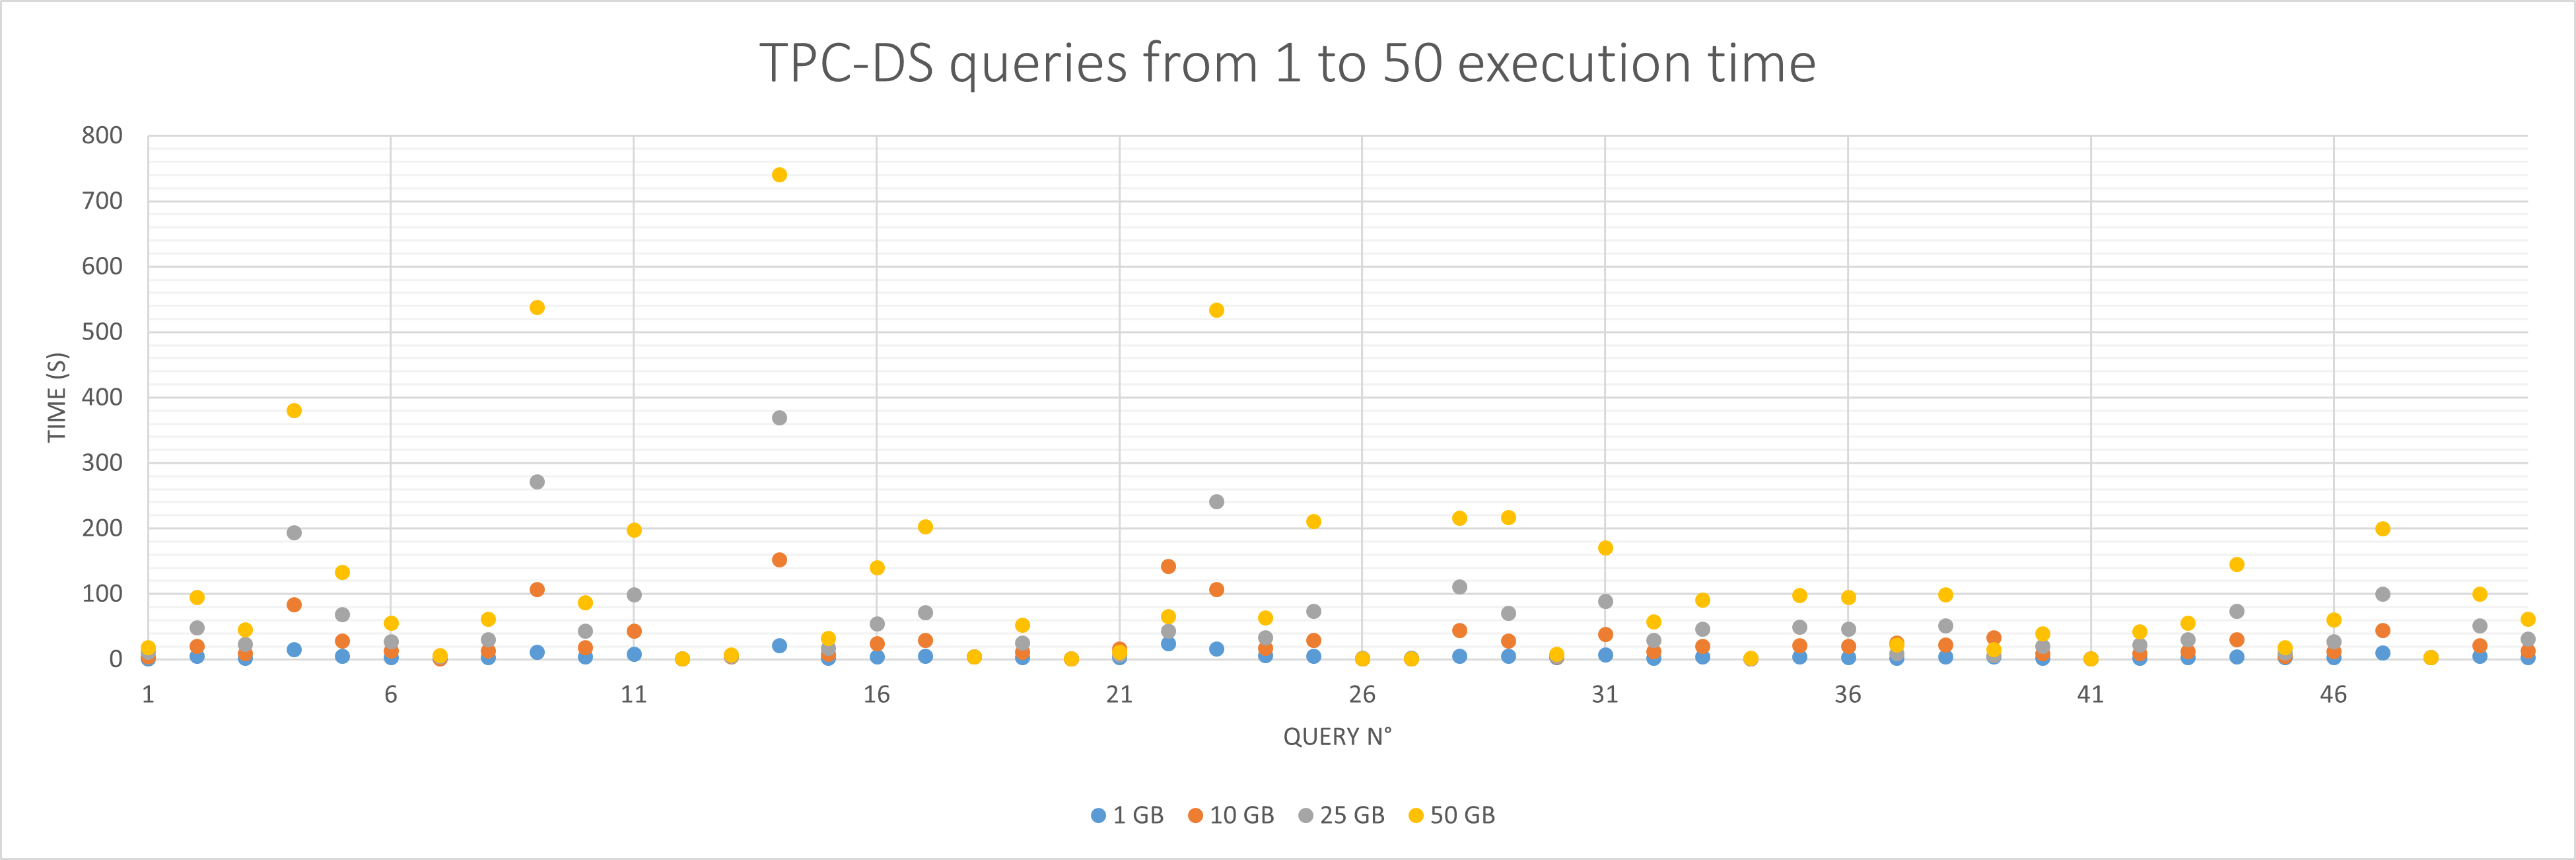
\includegraphics[width=20cm]{images/ExecutionTime1-50.png}
\end{center}
\end{adjustwidth}
\caption{Execution time of queries from 1 to 50}
\label{ExecutionTime1-50}
\end{figure}

\begin{figure}[H] 
\begin{adjustwidth}{-2cm}{-2cm}
\begin{center}
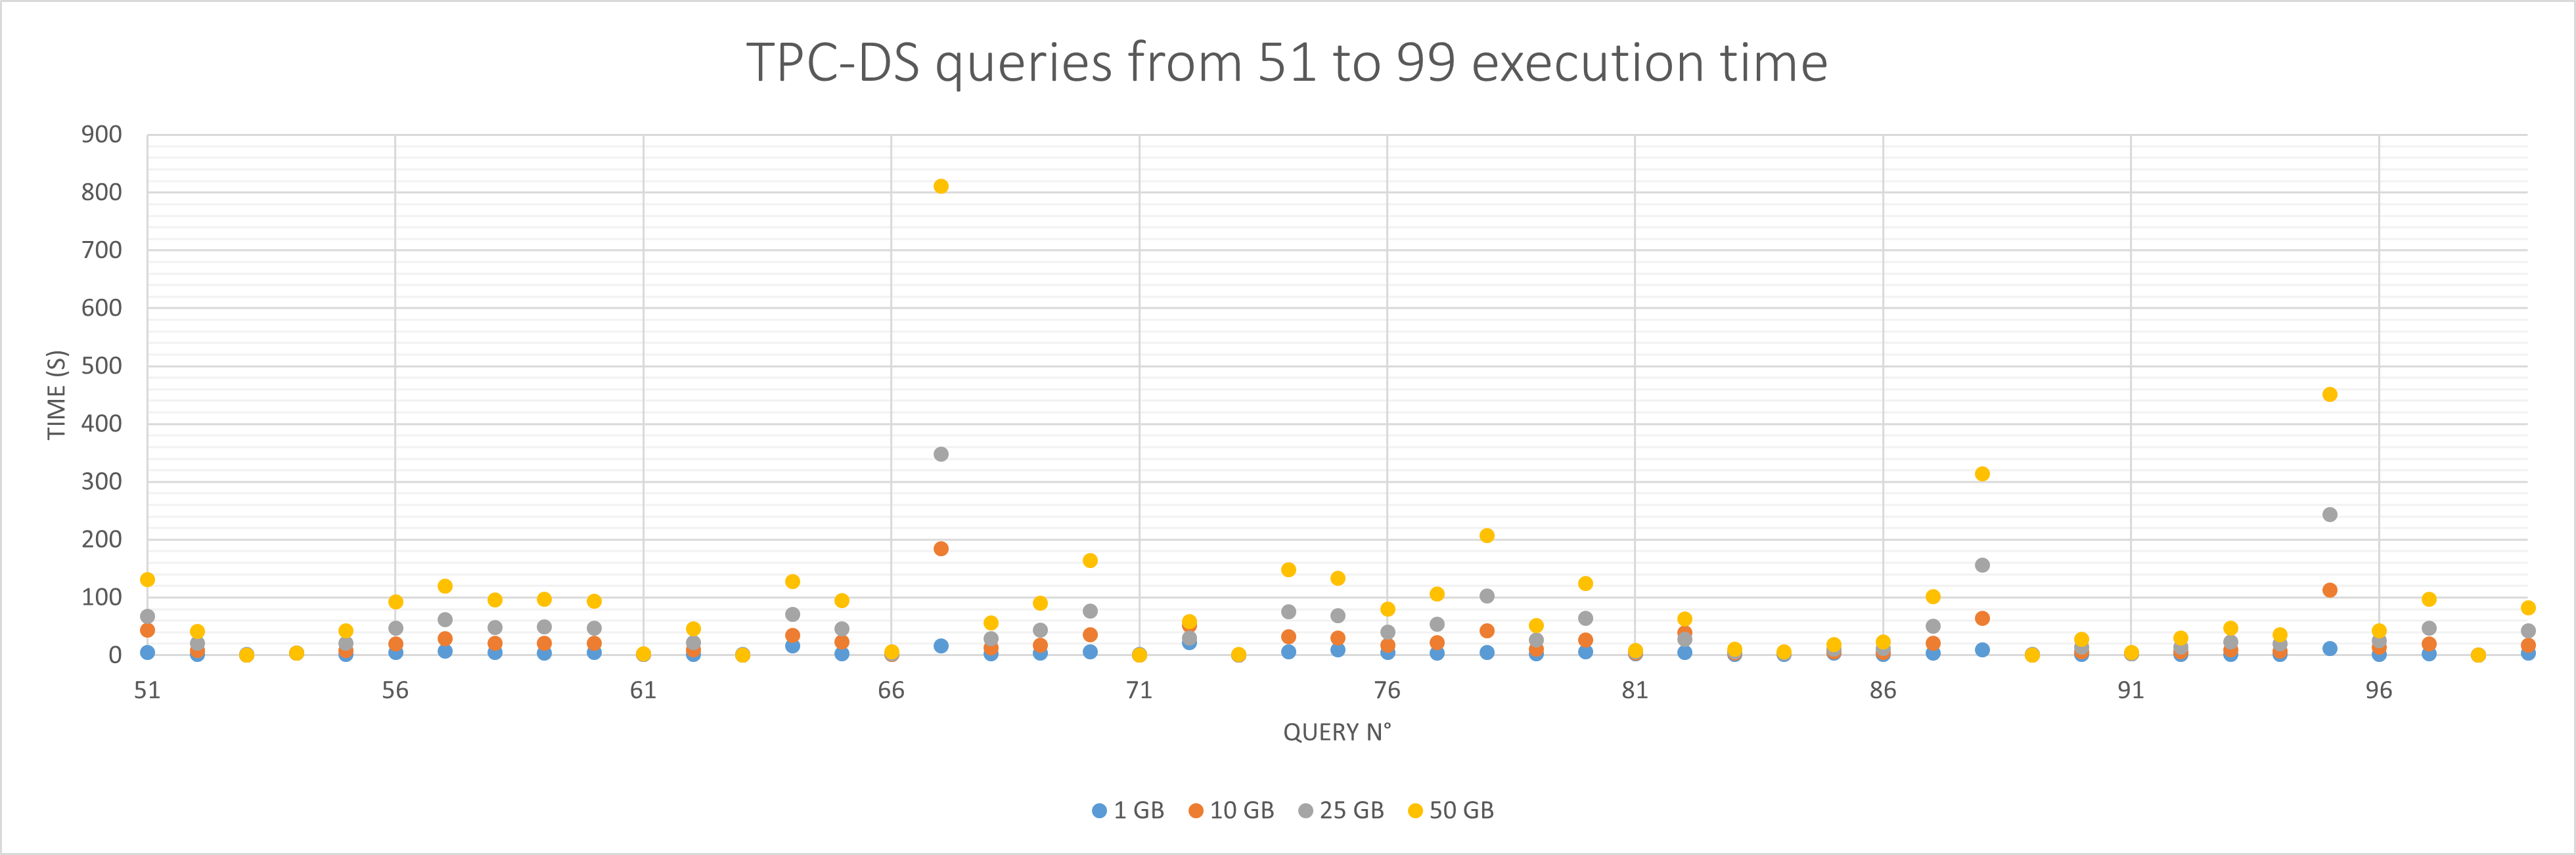
\includegraphics[width=20cm]{images/ExecutionTime51-99.png}
\end{center}
\end{adjustwidth}
\caption{Execution time of queries from 51 to 99}
\label{ExecutionTime51-99}
\end{figure}

The queries where only the yellow bullet can be seen, are queries where the size of the database has a negligible impact.

The results of the query 22 seem to be inconsistent, as it takes longer for it to complete with 10 GB of data than all the other scale. It can be explained as the queries are generated for a specific scale factor as described in TPC-DS documentation.

Some queries are highly dependent on the size of the data they operate on. Especially the following ones :

\begin{itemize}
    \item Query 4 : It has a lot of \textbf{union all}'s. Which means that more than one table is included on the operations, which adds a non-negligible execution time.
    \item Query 9 : It has a lot of cases. The same operation has been repeated with different parameters, which means that the used table has been read many times.
    \item Query 14 : It has a lot of \textbf{intersect}'s, indeed the operation becomes more costly depending on the dataset size.
    \item Query 23 : It has a lot of \textbf{union all}'s and multiple nested \textbf{select}'s. Thus, the operation is more complex and a possible query optimization can improve the time of execution.
    \item Query 67 : It has a nested \textbf{select}'s with depth of 3.
    \item Query 95 : It has more than one \textbf{select} in a where statement. As a consequence, the \textbf{where} clause becomes more costly to verify, thus doing that twice is time-consuming.
\end{itemize}


\subsection{Execution time growth}

The following graph \ref{ExecutionTimeGrowth} shows the growth of execution time of all the queries compared to the size of the datasets. Notice that the execution time is calculated as the overall sum of the time execution of each query independently, and not the real time needed to execute all of them on the computer. These two values can be different due to different I/O operations used in the script.

\begin{figure}[H] 
\begin{center}
\includegraphics[width=15cm]{images/ExecutionTimegrowth.png}
\end{center}
\caption{Execution time growth}
\label{ExecutionTimeGrowth}
\end{figure} 


It can be seen in the graph \hyperref[ExecutionTimeGrowth]{7}, the growth of the execution time of all the queries compared to the size of the datasets, is linear. It means that Impala handles well queries which ran on large amount of data. Furthermore, a line can be traced which pass through all the points. This line can be used to extrapolate higher values of data sizes. As the points are not perfectly aligned, the method of least square has been used to get its equation.

Here is its equation :

$$y = 3.169x + 5.859$$


The function can be seen in the following graph \ref{ExecutionTimeGrowthPrediction} with the dotted line.

\begin{figure}[H] 
\begin{center}
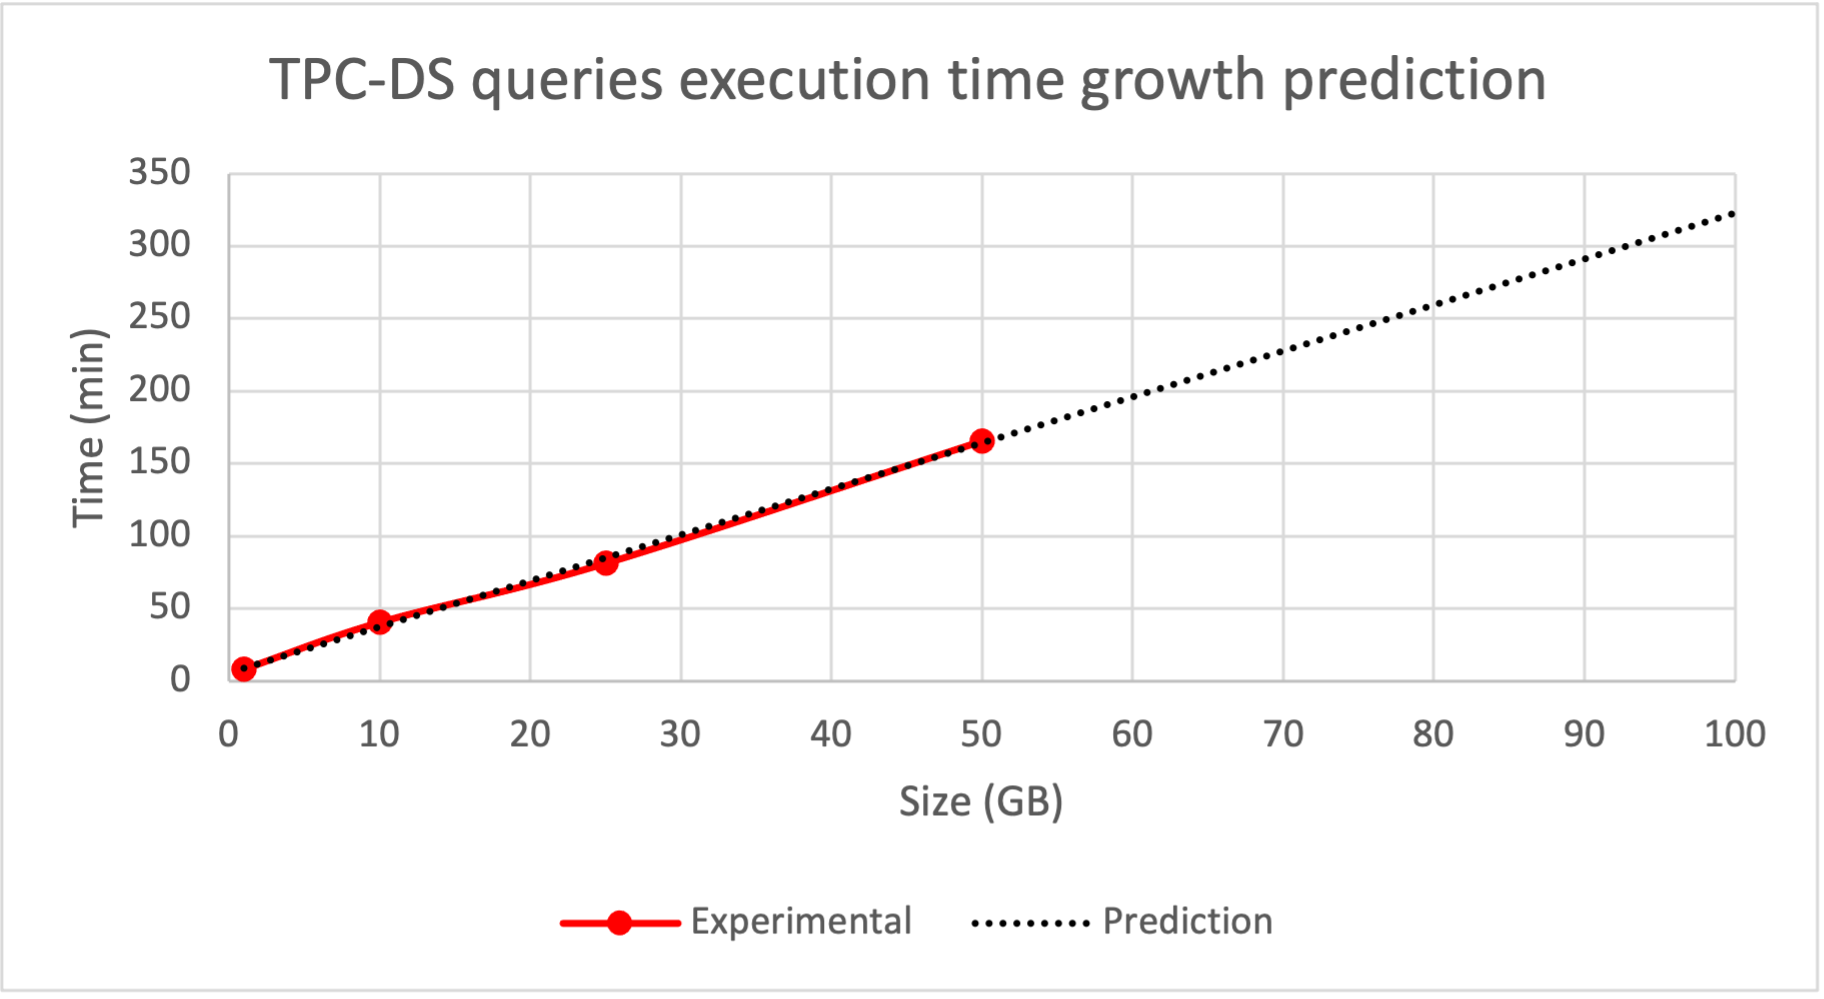
\includegraphics[width=15cm]{images/image.png}
\end{center}
\caption{Execution time growth prediction}
\label{ExecutionTimeGrowthPrediction}
\end{figure}

It means that for 100 GB of data, it is expected to get an execution time of 322.759 minutes.

%According to the datasets size, Impala's execution time was \bld{2.66} times quicker than the one which was expected. This value has been calculated by dividing the slope of the expectation function, by the slope of the experimentation output, which has been computed itself with the help of \bld{least square method}. This optimization factor, have been led to about \bld{60\%} of efficiency for Impala. It is quite surprising as the expected result was more of a logarithmic or a quadratic function.




\section{Conclusion}
In this project, \ita{TPC-DS} tools have been used in order to get a benchmark of Apache Impala. In this report, all the necessary steps were described in order for anyone to be able to reproduce the obtained results.

The first parts of this project were centered on the definitions of the different tools used. Additionally, all the steps needed for anyone to be able to install, launch and use Impala were fully detailed.

After that, the directives used to get the required materials, which were composed of the queries and the datasets, were seen. As all queries of \ita{TPC-DS} were not directly compatible with Impala, some of these queries have been syntactically altered and some were replaced by official alternatives one, so that they all could be executed via Impala.

As the diagrams of previous chapters show, it can be seen that the execution time increases with the size of the data, not exponentially but linearly. It can be assessed that Impala is indeed designed for large data warehouses, as it is capable of holding terabytes of data.

To sum up, it seems that Impala results are satisfying, even though very large datasets have not been tested because of the lack of resources.



\begin{thebibliography}{99}
    \bibitem{source001}
     \emph{Transaction Processing Performance Council (TPC), TPC BENCHMARK™ DS Standard Specification — Version 3.2.0, June 2021}
    
\end{thebibliography}

\end{document}
